To evaluate the accuracy of the \osprey \ks algorithm, we performed a series of designs for a variety of protein-protein interfaces. We used \ks to computationally predict experimentally measured effects on binding for each system. These systems include barnase with its peptide inhibitor barstar, the cytochrome {\it c}/cytochrome {\it c} peroxidase complex, interferon (IFN)$\alpha$2 with its receptor, ifnar2, the interleukin 2 (IL-2)/IL-2 receptor $\alpha$ (IL-2R$\alpha$) complex, and an antibody fragment bound to the I-domain of the integrin VLA1. 


Of the reported mutations, for our study we only included mutations proximal to the interface. Each design included one or two mutable positions along with a set of surrounding flexible residues. For each system, the \ks scores were ranked in increasing order of experimental binding. Spearman correlations were subsequently calculated for each system by calculating the Pearson correlation between the \ks score rankings and the experimentally measured rankings. 

\begin{table}[h!]
\centering
\begin{tabular}{ |c||c|  }
 \hline
 \textbf{System (PDB ID)}& \textbf{Spearman correlation} \\
 \hline 
 1X1U   & 0.755 \\
 \hline
 2B5I   & 0.519 \\
 \hline
 2PCB   & 0.500 \\
 \hline
 3S9D   & 0.795 \\
 \hline
 1MHP   & 0.365 \\
 \hline 
 \textbf{Across Systems} &   \textbf{0.632}  \\
 \hline
\end{tabular}
\caption{Spearman correlation table.}
\end{table}

\begin{figure}\label{fig:rankings}
\center
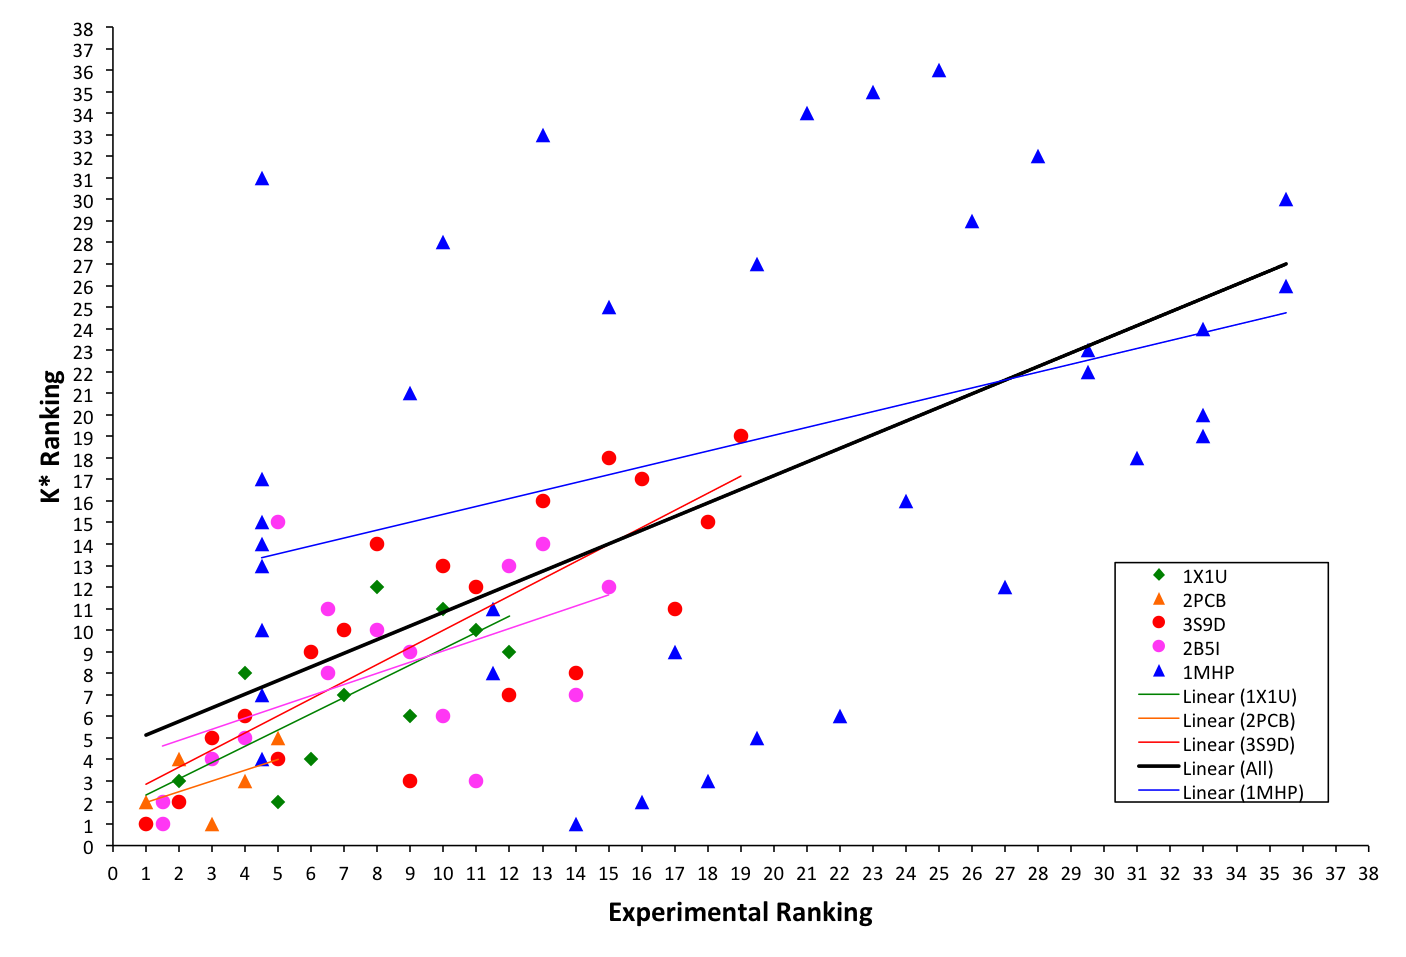
\includegraphics[width=0.9\textwidth]{figures/Rankings.png}
\caption{Testing the accuracy of \osprey3.}
\end{figure}

